\chapter{Kinematic model} \label{sec:kinematic-model}

This thesis is mainly concerned with the scanner system and the control of it's movement. However, to understand how the movement of the scanner system influences the print, some other components are necessary to consider as well. The laser must obviously be taken into account, but also the f-theta lens is important to consider since the laser passes through it after it has been steered by the scanner. The interaction of scanner, laser and f-theta lens  will be combined in a mathematical model to understand the relation between the movement of the scanner mirrors and the intersection of the laser with the image plane, ie. the position of the melt pool on the build plate. The angles of the scanner mirrors are considered the input to the kinematic model, and the position of the melt pool is considered the output. While the model of the individual parts are interesting in their own right, the main goal of this model is to express this output as a function of only the input and known constants. This function will be considered the forward kinematic equation of the L-PBF system.

Even though a laser beam is not classically a part of a kinematic model, the method used in this chapter to describe its path is the same. A geometrical optics approach is taken, where the laser beam is represented by a single straight line. In reality the beam is expanded before entering the scanner system and then focused again by the f-theta lens. For this simplified model however, it is sufficient to consider only the centre of the expanded beam, since this will yield the correct focus position of the laser in the image plane \cite{geometrical-optics}. The model will neither consider power loss of the laser in the mirrors nor in the lens.

The model is constructed in a regular right-hand Cartesian coordinate system with the xy-plane aligned with the image plane of the L-PBF system. The image plane in the L-PBF system means the plane in $\mathbb{R}^3$ containing the powder bed. Origo is taken to be where the laser points when both scanner mirrors are in their middle position, and the z-axis is oriented upwards from the image plane. A plot of the completed model can be seen on Figure \ref{fig:kin-model}. The model is constructed by first assuming the mirrors to be in their middle position, backtracking the path of the laser to determine the placement and rotation of the mirrors and the f-theta lens. Then, the laser path is calculated starting from the laser source and a parametric representation for each segment is found based on the angle of the mirrors, and the effect of the lens. The forms of the various parametric representations used throughout this chapter are based on Reference \cite{mat1-efterår}. The constants and variables used in the construction of the model are listed in Tables \ref{tab:model-constants} and \ref{tab:model-vars}. The dimensions are chosen to correspond as closely as possible with the specifications of the actual components used in Baxter (see References \cite{scanner-spec} and \cite{f-theta-lens-spec}).

\begin{figure}[p]
    \centering
    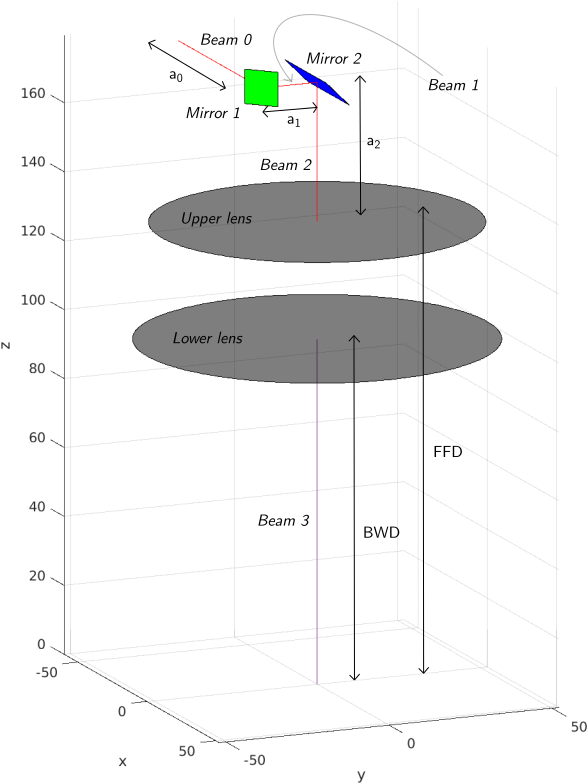
\includegraphics[width=\linewidth]{Pictures/kin-model.png}
    \caption{Plot of all the components of the kinematic model. FFD and BWD are reduced to a fifth of the actual lenghts for readability. Upper lens and lower lens represent the upper and lower surface of the f-theta lens. The units on all axis are mm.}
    \label{fig:kin-model}
\end{figure}

\begin{table}[H]
    \centering
    \begin{tabular}{l|c|c|p{100mm}}
        Symbol  & Value & Unit  & Description \\ \hline
        $l_1$   & 10    & mm    & Length of mirror 1 \\
        $w_1$   & 10    & mm    & Width of mirror 1 (the diameter of the rotation) \\
        $l_2$   & 30    & mm    & Lenght of mirror 2 \\
        $w_2$   & 10    & mm    & Width of mirror 2 (the diameter of the rotation) \\
        $r_u$   & 47.5  & mm    & Radius of the upper(/entrance) surface of the f-theta lens \\
        $r_l$   & 52    & mm    & Radius of the lower(/exit) surface of the f-theta lens \\
        $a_0$   & 70    & mm    & Distance from the laser source to the centre of mirror 1 \\
        $a_1$   & 17    & mm    & Distance between the centres of mirror 1 and mirror 2 \\
        $a_2$   & 40.5  & mm    & Distance from mirror 2 to the image plane \\
        $a_{FFD}$ & 534.1 & mm  & Distance from the upper surface of the f-theta lens to the image plane (Flange Focal Distance)\\
        $a_{BWD}$& 500.2 & mm    & Distance from the lower surface of the f-theta lens to the image plane (Back Working Distance)\\
        $\alpha_{EFL}$ & 423 & mm rad$^{-1}$ & Linear coefficient for the f-theta characteristic of the lens (Effective Focal Length)\\
    \end{tabular}
    \caption{Constants used in the mathematical model of the scanner system}
    \label{tab:model-constants}
\end{table}

\begin{table}
    \centering
    \begin{tabular}{l|c|l}
        Symbol      & Unit  & Description \\ \hline
        $\theta_1$  & rad.  & Angle of mirror 1, determining the x-coordinate of the melt pool ($s_x$) \\
        $\theta_2$  & rad.  & Angle of mirror 2, determining the y-coordinate of the melt pool ($s_y$)
    \end{tabular}
    \caption{Variables used in the mathematical model of the scanner system}
    \label{tab:model-vars}
\end{table}

\section{Mirrors}

Both mirrors are modelled by parametric plane equations. Firstly, axis parameters for a plane are chosen, then rotation is considered, and lastly the centre position is shifted to match the laser path. The model has to be constructed in this order, since the rotation influences the centre position and would move the mirror away from the correct position if it was incorporated into the model in the end.

Mirror 2 is constructed first. The basis for modelling this mirror is a parametric equation for the xz-plane that represents the mirror surface and can be seen in Equation \ref{eq:p2} where $s_2$ is the width-parameter and $t_2$ the length-parameter

\begin{align}
    p_{2} &=
    t_2
    \begin{bmatrix}
        1 \\
        0 \\
        0 \\
    \end{bmatrix}
    +
    s_2
    \begin{bmatrix}
        0 \\
        0 \\
        1 \\
    \end{bmatrix}
    \quad , \quad
    s_2 \in \left[\frac{-w_{2}}{2}, \frac{w_{2}}{2}\right] \vee 
    t_2 \in \left[\frac{-l_{2}}{2}, \frac{l_{2}}{2}\right]
    \label{eq:p2}
\end{align}

Mirror 2 adjusts the y-position of the melt pool by rotating around the x-axis. The corresponding rotation matrix is represented by Equation \ref{eq:r2} where $\theta_2$ is the mirror angle. $\pi/4$ radians is the neutral position, that points the laser at y=0.

\begin{align}
    R_{x}(\theta_1) &=
    \begin{bmatrix}
        1           & 0             & 0             \\
        0           & cos(\pi/4 + \theta_2)   & -sin(\pi/4 + \theta_2)  \\
        0           & sin(\pi/4 + \theta_2)   & cos(\pi/4 + \theta_2)   \\
    \end{bmatrix}
    \label{eq:r2}
\end{align}

By following the laser path backwards from the origo, the centre of the mirror is found to be as represented in Equation \ref{eq:c2}

\begin{align}
    c_{2} &=
    \begin{bmatrix}
        0 \\
        0 \\
        a_{2} + a_{FFD} \\
    \end{bmatrix}
    \label{eq:c2}
\end{align}

The plane equation, rotation matrix and position vector can then be combined to give the full equation for the mirror as a function of $\theta_2$. 

\begin{align}
    m_{2}(\theta_2) &= R_{x}(\theta_2) p_{2} + c_{2}
\end{align}

Mirror 1 is modelled in similar fashion, this time also starting with the y=0 plane, as described in Equation \ref{eq:p1}.

\begin{align}
    p_{1} &=
    s_1
    \begin{bmatrix}
        1 \\
        0 \\
        0 
    \end{bmatrix}
    +
    t_1
    \begin{bmatrix}
        0 \\
        0 \\
        1 
    \end{bmatrix}
    \quad , \quad
    s_1 \in \left[\frac{-w_1}{2}, \frac{w_1}{2}\right] \vee 
    t_1 \in \left[\frac{-l_1}{2}, \frac{l_1}{2}\right]
    \label{eq:p1}
\end{align}

The rotation matrix for mirror 1 (described in Equation \ref{eq:r1}) is rotating the mirror around the z-axis. This rotation ends up determining the x-position of the melt pool. The neutral postion is $\pi/4$ radians which points the laser to x=0. The mirror angle $\theta_1$ is subtracted instead of added to make increase in $\theta_1$ correspond to increase in x-value in the image plane.

\begin{align}
    R_{z}(\theta_1) &=
    \begin{bmatrix}
        cos(\pi/4 - \theta_1)   & -sin(\pi/4 - \theta_1)& 0             \\
        sin(\pi/4 - \theta_1)   & cos(\pi/4 - \theta_1) & 0             \\
        0                       & 0                     & 1 
    \end{bmatrix}
    \label{eq:r1}
\end{align}

The centre position of mirror 1 is found by adding the offset caused by laser segment 2 and laser segment 1 and is represented as a vector in Equation \ref{eq:c1}

\begin{align}
    c_{1} &=
    \begin{bmatrix}
        0       \\
        -a_{1}  \\
        a_{2} + a_{FFD}
    \end{bmatrix}
    \label{eq:c1}
\end{align}

Combining plane, rotation and offset gives Equation \ref{eq:m1} which describes mirror 1 as a function of $\theta_1$.

\begin{align}
    m_{1}(\theta_1) &= R_{z}(\theta_1) p_{1} + c_{1}
    \label{eq:m1}
\end{align}

\section{F-theta Lens} \label{sec:f-theta-model}

The f-theta lens is placed between mirror 2 and the image plane. The lens will be modelleld as two discs both parallel to the image plane and centered at (x,y) = (0,0). The upper disc represents the entrance surface of the lens and has $z=a_{FFD}$. The lower disc represents the exit surface of the lens and has $z=a_{BWD}$. Even though the surfaces in reality are curved, they are represented as flat surfaces in this model.

The parametric equations for the discs are obtained by adding the centre offsets to parametric discs in the xy-plane as shown in Equations \ref{eq:du} and \ref{eq:dl}.

\begin{align}
    d_u &=
    t_u
    \begin{bmatrix}
        cos(v_u) \\
        sin(v_u) \\
        0 \\
    \end{bmatrix}
    +
    \begin{bmatrix}
        0 \\
        0  \\
        a_{FFD} \\
    \end{bmatrix}
    \quad , \quad
    t_u \in \left[0, r_u\right] \vee 
    v_u \in \left[0, 2\pi\right[
    \label{eq:du} \\
    d_l &=
    t_l
    \begin{bmatrix}
        cos(v_l) \\
        sin(v_l) \\
        0 \\
    \end{bmatrix}
    +
    \begin{bmatrix}
        0 \\
        0  \\
        a_{BWD} \\
    \end{bmatrix}
    \quad , \quad
    t_l \in \left[0, r_l\right] \vee 
    v_l \in \left[0, 2\pi\right[
    \label{eq:dl}
\end{align}

F-theta lenses are intricate optical devices that influence the laser path in very complex ways. Often the exact designs are proprietary and their operation can, if anything, only be assessed by a black box model supplied by the manufacturer of the lens \cite{thorlabs-ftheta}. The main purpose of f-theta lenses is to focus the (previously expanded) laser beam on a flat surface, namely the image plane. This effect is not included in the present mathematical model since the width of the beam is not considered. The other purpose of the f-theta lens is to establish a linear relation between the incidence angle of the laser and the position in the image plane. This is also what gives the lens it's name: f for Focal Length and theta for the incidence angle. This linear relation is represented in Equations \ref{eq:f-theta-x} and \ref{eq:f-theta-y} where s is the position in the image plane, $\alpha_{EFL}$ is the Effective Focal Length, a lens-specific linear coefficient, and $\theta$ is the incidence angle of the laser on the lens. The incidence angles turn out to be twice the mirror angles, so $\theta_x = 2\theta_1$ and $\theta_y = 2\theta_2$ as will be illustrated on Figure \ref{fig:v1}. The effective focal length is normally denoted as $f$ but $\alpha_{EFL}$ is used here to avoid confusion with later function definitions.

\begin{align}
    s_x &= \alpha_{EFL} \theta_x \label{eq:f-theta-x} \\
    s_y &= \alpha_{EFL} \theta_y \label{eq:f-theta-y}
\end{align}

These are the equations that will be used in this model to describe how the lens influences the path of the laser. The laser will be assumed to exit the f-theta lens in the same (x, y)-coordinates as it enters.

\section{Laser}

The laser will be modelled by dividing it into seperate line segments. Each beam segment represents a piece of the laser going between two other elements of the model, as previously shown on Figure \ref{fig:kin-model}. The equations for the beam segments of the laser are determined by starting from the laser source and the beams are indexed in increasing order starting with beam segment 0 between the laser source and mirror 1. The position of the laser source is found by adding up all laser segments as shown in Equation \ref{eq:c0}.

\begin{align}
    c_0 =
    \begin{bmatrix}
        -a_0 \\
        -a_1 \\
        a_2 + a_{FFD}
    \end{bmatrix}
    \label{eq:c0}
\end{align}

For the beam segment 0 a parametric representation that describes the laser beam from the source to the first mirror is presented in Equation \ref{eq:b0}

\begin{align}
    b_0 = c_0 + u_0
    \begin{bmatrix}
        1 \\
        0 \\
        0 \\
    \end{bmatrix}
    \quad , \quad
    u_0 \in [0, \text{intersection with mirror 1}]
    \label{eq:b0}
\end{align}

The intersection of beam 0 with mirror 1, $m_1'$ is found be solving Equation \ref{eq:m1int} for $u_0$, $s_1$ and $t_1$, and substituting back into either of the expressions.

\begin{align}
    m_1 = b_0
    \label{eq:m1int}
\end{align}

A normal vector of $m_1$ is used to find the reflection of $b_0$ in $m_1$. This normal vector is obtained by calculating the cross product of the two component vectors, as shown in Equation \ref{eq:n1}.

\begin{align}
    n_1 = \left( R_z
    \begin{bmatrix}
        1 \\
        0 \\
        0
    \end{bmatrix} \right)
    \times
    \left( R_z
    \begin{bmatrix}
        0 \\
        0 \\
        1
    \end{bmatrix} \right)
    \label{eq:n1}
\end{align}

Then the projection of the beam onto the normal vector is found in Equation \ref{eq:proj-b0-n1}

\begin{align}
    proj(b_0, n_1) = \frac{n_1 \cdot (c_0 - m_1')}{|n-1|^2} n_1 \label{eq:proj-b0-n1}
\end{align}

Now, it's possible to construct the direction vector for the section 1 of the laser by constructing a vector from the mirror image of the laser source in mirror 1 to the intersection point of beam 0 with mirror 1. This is described in Equation \ref{eq:v1} and shown graphically on Figure \ref{fig:v1}. On this figure it is also important to notice that $\theta_x$, the deflection angle in the x-direction, is double $\theta_1$, as described in Equations \ref{eq:theta-x-1} and \ref{eq:theta-y-2} (The same holds true for $\theta_y$ and $\theta_2$).

\begin{align}
    \theta_x = 2\theta_1 \label{eq:theta-x-1}\\
    \theta_y = 2\theta_2 \label{eq:theta-y-2}
\end{align}

\begin{align}
    v_1 = m_1' - (c_0 - 2proj(b_0, n_1))
    \label{eq:v1}
\end{align}

\begin{figure}[t]
    \centering
    \includesvg[width=0.9\linewidth]{Pictures/proj-explain-text-to-path.svg}
    \caption{A graphic explanation of Equation \ref{eq:v1}.}
    \label{fig:v1}
\end{figure}

At this point everything is ready to construct segment 1 of the laser as shown in Equation \ref{eq:b1}.

\begin{align}
    b_1 = m_1' + u_1 v_1 \quad , \quad u_1 \in [0, \text{intersection with mirror 2}] \label{eq:b1}
\end{align}

Segment 2 is done similarly. The laser intersection with mirror 2, $m_2'$ is found by solving Equation \ref{eq:m2int} for $u_1$, $s_2$ and $t_2$, and then substituting back into either $m_2$ or $b_1$

\begin{align}
    m_2 = b_1
    \label{eq:m2int}
\end{align}

Once more the normal vector is calculated (see Equation \ref{eq:n2})

\begin{align}
    n_2 = \left( R_x
    \begin{bmatrix}
        1 \\
        0 \\
        0
    \end{bmatrix} \right)
    \times
    \left( R_x
    \begin{bmatrix}
        0 \\
        0 \\
        1
    \end{bmatrix} \right)
    \label{eq:n2}
\end{align}

And the projection of section 1 of the laser on the normal vector of mirror 2 is constructed (see Equation \ref{eq:proj-b1-n2}).

\begin{align}
    proj(b_1, n_2) = \frac{n_2 \cdot (m_1' - m_2')}{|n_2|^2} n_2
    \label{eq:proj-b1-n2}
\end{align}

The direction vector for section 2 of the laser is now found. This is again done with the mirror image, but this time instead of the laser source, it's the intersection with mirror 1, mirrored in mirror 2 as noted in Equation \ref{eq:v2}

\begin{align}
    v_2 = m_2' - (m_1' - 2proj(b_1, n_2)) \label{eq:v2}
\end{align}

The direction vector $v_2$ and the position vector $m_2'$ can then be combined into laser segment 2 like shown in Equation \ref{eq:b2}.

\begin{align}
    b_2 = m_2' + u_2 v_2 \quad , \quad u_2 \in [0, \text{intersection with upper lens surface}] \label{eq:b2}
\end{align}

Beam 3 is calculated differently from the other segments because its direction is determined by the f-theta lens rather than a mirror. Still, the first step is to find the intersection of beam 2 with the upper lens surface by solving Equation \ref{eq:pu-int} for x and y.

\begin{align}
    p_{u}' =
    \begin{bmatrix}
        x \\
        y \\
        a_{FFD}
    \end{bmatrix}
    \label{eq:pu-int}
\end{align}

It is then assumed that the beam exits the lower surface of the lens at the same (x,y)-coordinates. This assumption leads to Equation \ref{eq:plm}.

\begin{align}
    p_{l}' = p_{u}' + 
    \begin{bmatrix}
        0 \\
        0 \\
        a_{BWD} - a_{FFD}
    \end{bmatrix}
    \label{eq:plm}
\end{align}

This is not a very accurate assumption, but it's workable and inconsequential for the purpose. The next step is to simply find the position of the melt pool (the intersection of beam 3 with the image plane) from the f-theta equations and combine them to a vector which is done in Equation \ref{eq:xy-int}.

\begin{align}
    p_{xy}' =
    \begin{bmatrix}
        \alpha_{EFL} \theta_x \\
        \alpha_{EFL} \theta_y \\
        0
    \end{bmatrix}
    \label{eq:xy-int}
\end{align}

Now the direction vector for beam 3 is constructed in Equation \ref{eq:v3} by pointing it from one end of beam 3 to the other.

\begin{align}
    v_3 = p_{xy}' - p_u' \label{eq:v3}
\end{align}

Beam 3 can then be described by the parametric representation in Equation \ref{eq:b3}.

\begin{align}
    b_3 = p_u' + u_3 v_3 \quad,\quad u_3 \in [0, \text{intersection with image plane}] \label{eq:b3}
\end{align}

This concludes the modelling of all the individual parts of the kinematic model.

\section{Forward kinematic model results}
What the above derivations show is, that the main equations describing the system from beginning to end are actually given mostly by the f-theta lens and less by the scanner geometry. The f-theta lens gives the relations presented in Equations \ref{eq:f-theta-x} and \ref{eq:f-theta-y} (reproduced here for readability)

\begin{align}
    s_x = \alpha_{EFL} \theta_x \tag{\ref{eq:f-theta-x}} \\
    s_y = \alpha_{EFL} \theta_y \tag{\ref{eq:f-theta-y}}
\end{align}

The only thing that must be known about the scanner is how the mirror angles relates to the incidence angle of the f-theta lens. This was expressed in Equations \ref{eq:theta-x-1} and \ref{eq:theta-y-2} (reproduced here for readability)

\begin{align}
    \theta_x = 2\theta_1 \tag{\ref{eq:theta-x-1}} \\
    \theta_y = 2\theta_2 \tag{\ref{eq:theta-y-2}}
\end{align}

Theses four equations can then be combined to define the full forward kinematic equations. The forward kinematic equations express the output of the model, ie. the displacement of the melt pool ($s_x, s_y$) as a function of the inputs to the model, ie. the mirror angles ($\theta_1, \theta_2$) and known constants. They are presented as Equations \ref{eq:forward-kin-x} and \ref{eq:forward-kin-y}.

\begin{align}
    s_x = 2\alpha_{EFL} \theta_1 \label{eq:forward-kin-x} \\
    s_y = 2\alpha_{EFL} \theta_2 \label{eq:forward-kin-y}
\end{align}

Even though it is the f-theta relations that mostly define the forward kinematic equations, the other parts of the model are important for be explaining why these equations, while very accurate, are only approximations.

\section{Deviations from the f-theta equations} \label{sec:f-theta-dev}

The real behaviour of the function from $\theta_1$ and $\theta_2$ to $s_x$ and $s_y$ deviates from the idealised f-theta equations in two main ways: Difference in deflection angle and naive split in x- nad y-angle

\subsection{Difference in deflection distance} \label{sec:f-theta-dev-dist}
The f-theta lens is constructed in a way that the relation holds only for beams being deflected at a certain distance from the lens. This becomes clear by the following thought experiment: Imagine if the scanner was moved farther away from the lens. This would mean that the laser would enter the lens at a different position, resulting in a different position of the melt pool \textit{even though the mirror angle is the same}. This shows clearly that the f-theta relation only holds when there is a certain specified distance between the mirror and the lens. The problem with this is, that the angles in x-direction and y-direction \textit{are} deflected at different distances from the lens ($a_1+a_2$ and $a_2$ respectively), and the lens cannot be perfect for both \cite{ftheta-hard}. Because of this, the mirrors are placed as close together as possible in the scanner. Furthermore manufacturers of f-theta lenses might use heuristic optimisations to compensate for the resulting error, but still this observation leads to the possibility that the actual $\alpha_{EFL}$ might be different for x and y.

\subsection{Naive split in x- and y-angle} \label{sec:f-theta-dev-angle}
The f-theta characteristic is in fact only one equation and can only as an approximation be split into two independent equations for each of the coordinates like it is done in this model \cite{correction-cals}. In the original f-theta relation $\theta$ means the angle between the beam and the $x=y=0$ line, and the distance $s_r$ is the distance to the centre of the image plane\cite{thorlabs-ftheta}. This original relation is presented in Equation \ref{eq:f-theta-r}.
\begin{align}
    s_r = \alpha_{EFL} \theta_r
    \label{eq:f-theta-r}
\end{align}

If only one of the mirrors is not in it's middle position, this original relation and the coordinate-split versions are the same. The problem arises when both mirror angles are different from their middle position, because angles don't add up like distances. The distances add up by Pythagoras theorem (Equation \ref{eq:sx-sy-sr}).

\begin{align}
    s_r = \sqrt{s_x^2 + s_y^2}
    \label{eq:sx-sy-sr}
\end{align}
    
Substituting in the angles with the respective f-theta relations produces Equation \ref{eq:theta-x-y-r-wrong} which is not true generally.
    
\begin{align}
    \alpha_{EFL} \theta_r &= \sqrt{(\alpha_{EFL} \theta_x)^2 + (\alpha_{EFL} \theta_y)^2} \\
    \alpha_{EFL} \theta_r &= \sqrt{\alpha_{EFL}^2(\theta_x^2 + \theta_y)^2} \\
    \alpha_{EFL} \theta_r &= \alpha_{EFL} \sqrt{\theta_x^2 + \theta_y^2} \\
    \theta_r &= \sqrt{\theta_x^2 + \theta_y^2} \qquad \text{\huge \Lightning} \label{eq:theta-x-y-r-wrong}
\end{align}
    
The true relations can be derived from Figure \ref{fig:theta-s-plot}.
    
\begin{figure}[ht]
    \centering
    \includesvg[width=0.75\linewidth]{Pictures/theta-s-plot.svg}
    \caption{Plot showing how $\theta_x$, $\theta_y$ and $\theta_r$ relate. This figure ignores the fact that angles $\theta_x$ and $\theta_y$ aren't deflected at the same position in the actual system. In other words it assumes $a_1 = 0$}
    \label{fig:theta-s-plot}
\end{figure}
    
This figure shows that the relation of $\theta_r$ to $\theta_x$ and $\theta_y$ is in fact like described in Equation \ref{eq:theta-s-true}.
    
\begin{align}
    a_2 tan(\theta_r) &= \sqrt{(a_2 tan(\theta_x))^2 + (a_2 tan(\theta_y))^2} \\
    tan(\theta_r) &= \sqrt{tan(\theta_x)^2 + tan(\theta_y)^2}
    \label{eq:theta-s-true}
\end{align}
    
Note that this equation reduces to equation \ref{eq:theta-x-y-r-wrong} if either $\theta_x = 0$ or  $\theta_y = 0$ and approximates it for small angles because of the small angle approximation $tan(\theta) = \theta$. The conclusion to this is, that even if it is assumed that the f-theta lens follows Equation \ref{eq:f-theta-r} perfectly, the coordinate-by-coordinate Equations \ref{eq:f-theta-x} and \ref{eq:f-theta-y} are not completely true but only approximations. The manufacturer might also use heuristic design modifications to compensate for this fundamental problem. Still this observation goes to show that the movements in x and y directions aren't completely independent, as the f-theta equations would otherwise suggest.

\section{Inverse and velocity kinematics}
The model presented in this chapter until now has described how the mirror angles $\theta_1$ and $\theta_2$, which are considered the input, are related to $s_x$ and $s_y$ the coordinates of the intersection of the laser with the image plane, which is considered the output. But an maybe even more relevant question is that of the inverse kinematic equations: given a desired $s_x$ and $s_y$, what values for $\theta_1$ and $\theta_2$ will result in this output? The f-theta lens makes it trivial to find both the inverse and velocity kinematics for the system. The inverse kinematic equations are found by solving Equations \ref{eq:forward-kin-x} and \ref{eq:forward-kin-y} for $\theta_1$ and $\theta_2$. The resulting inverse kinematic equations are presented in Equations \ref{eq:inv-kin-x} and \ref{eq:inv-kin-y}. 

\begin{align}
    \theta_1 &= \frac{s_x}{2\alpha_{EFL}} \label{eq:inv-kin-x} \\
    \theta_2 &= \frac{s_y}{2\alpha_{EFL}} \label{eq:inv-kin-y}
\end{align}

The velocity kinematics are found by taking the derivative on each side of Equations \ref{eq:forward-kin-x} and \ref{eq:forward-kin-y} with respect to time. The result is just that the position variables $s_x$ and $s_y$ are changed out for velocities $v_x$ and $v_y$ and the angle variables $\theta_1$ and $\theta_2$ become angular velocities $\omega_1$ and $\omega_2$. The velocity kinematics are shown in Equations \ref{eq:vel-kin-x} and \ref{eq:vel-kin-y}. Note that the velocity is not dependent on the position, which is often the case in other systems.

\begin{align}
    v_x &= 2\alpha_{EFL} \omega_1 \label{eq:vel-kin-x}\\
    v_y &= 2\alpha_{EFL} \omega_2 \label{eq:vel-kin-y}
\end{align}

All of the above modelling is an attempt to describe real the behaviour of the L-PBF system in a way that can be analysed and used to predict different scenarios. But it is also an idealised version of the system, a picture of how one would hope the system behaved. The real system can of course never be made to follow the idealised version completely, but calibration can help some way towards that goal.
